
% ===========================================================================
% Title:
% ---------------------------------------------------------------------------
% to create Type I fonts type "dvips -P cmz -t letter <filename>"
% ===========================================================================
\documentclass[11pt]{article}       %--- LATEX 2e base
\usepackage{latexsym}               %--- LATEX 2e base
%---------------- Wide format -----------------------------------------------
\textwidth=6in \textheight=9in \oddsidemargin=0.25in
\evensidemargin=0.25in \topmargin=-0.5in
%--------------- Algorithm --------------------------------------------------
\newtheorem{algX}{Algorithm}
\newenvironment{algorithm}       {\begin{algX}\begin{em}}%
                                 {\par\noindent --- End of Algorithm ---
                                 \end{em}\end{algX}}
\newcommand{\step}[2]            {\begin{list}{}
                                  {  \setlength{\topsep}{0cm}
                                     \setlength{\partopsep}{0cm}
                                     \setlength{\leftmargin}{0.8cm}
                                     \setlength{\labelwidth}{0.7cm}
                                     \setlength{\labelsep}{0.1cm}    }
                                  \item[#1]#2    \end{list}}
                                 % usage: \begin{algorithm} \label{xyz}
                                 %        ... \step{(1)}{...} ...
                                 %        \end{algorithm}
%--------------- Figures ----------------------------------------------------
\usepackage{graphicx}

\newcommand{\includeFig}[3]      {\begin{figure}[htb] \begin{center}
                                 \includegraphics
                                 [width=4in,keepaspectratio]
                                 {#2}\caption{\label{#1}#3} \end{center} \end{figure}}
                                 % usage: \includeFig{label}{file}{caption}


% ===========================================================================
\begin{document}
% ===========================================================================

% ############################################################################
% Title
% ############################################################################

\title{Accelerating Genetic ANN Training using the CUDA Platform}


% ############################################################################
% Author(s) (no blank lines !)
\author{
% ############################################################################
Catalin Patulea and Robert Peace\\
School of Systems and Computer Engineering\\
Carleton University\\
Ottawa, Canada K1S 5B6\\
{\em rpeace@sce.carleton.ca}
% ############################################################################
} % end-authors
% ############################################################################

\maketitle

% ############################################################################
% Abstract
% ############################################################################
\begin{abstract}
Filling this with text so that I can see what the document looks like when it is filled with text and to make sure that everything lines up nicely when it is full of text like this
\end{abstract}

% ############################################################################
\section{Introduction} \label{intro}
% ############################################################################
Artificial neural networks (ANNs) are a class of very flexible machine learning models applicable to many classification and regression tasks. All artificial neural networks share the same basic structure but their adaptability lies in the ability to vary the network topology, activation functions at each node, and the weights between each nodes. Together, these factors allow for a very comprehensive tool capable of modeling a wide range of systems.

Generally, for any given problem, the ANN designers choose a particular network structure. Then, during supervised learning, the labelled training instances are used to adjust the network parameters (edge weights and other node parameters) until some a given criteria is reached regarding classification error or training time. This can be seen as a search for a global minimum in the space of network parameters. Because the number of parameters in a typical neural network is in the tens or hundreds, the search is in a quite high-dimensional space and thus quite challenging.

The ANN parameter finding problem can be viewed as an optimization problem. Simple algorithms like the first order gradient descent, second-order Gauss-Newton or hybrid Levenberg�Marquardt rely on approximations of the error function to iteratively find the global extremum. These algorithms perform well when the error landscape is relatively simple, but for ANNs with complex structures and landscapes with many local extrema, they are susceptible to getting stuck at those local extrema and sometimes do not converge nicely. Additionally, they impose certain restrictions on the node function (differentiability).

Stochastic approaches to optimization provide some hope of escaping these shortcomings. One such example, simulated annealing, begins with a particular set of parameters and randomly perturbs them in the hopes of approaching an extremum. The new solution is chosen probabilistically, depending on a temperature parameter which decreases during this process. Thus, early during optimization we favor large-scale exploration of the search space while near the end we are exploring only the neighborhood of a particular local extremum (which we hope is the global extremum) to improve the precision of our solution.

Genetic algorithms (GAs) are stochastic optimization algorithms which try to leverage concepts of evolution and natural selection to find the optimal solution. Similarly to simulated annealing, GAs use random perturbations to explore the search space. However, GAs additioally operate on multiple solutions at a time and attempt to combine multiple partial solutions into a new better performing candidate. At the core of GAs is the definition of a "chromosome", which represents one candidate solution, as well as an associated set of genetic operators which perform domain-specific mutations on this candidate and enable candidate mating.

TODO: talk about GA resource-intensive (esp with ANN)
TODO: talk about CUDA being good for number-crunching
TODO: talk about CUDA performance dependent on memory access patterns

% ############################################################################
\section{Background} \label{background}
% ############################################################################
Filling this with text so that I can see what the document looks like when it is filled with text and to make sure that everything lines up nicely when it is full of text like this

% ----------------------------------------------------------------------------
\subsection{Artificial Neural Networks} \label{ann}
% ----------------------------------------------------------------------------
Filling this with text so that I can see what the document looks like when it is filled with text and to make sure that everything lines up nicely when it is full of text like this

% ----------------------------------------------------------------------------
\subsection{Genetic Algorithms} \label{ga}
% ----------------------------------------------------------------------------
Filling this with text so that I can see what the document looks like when it is filled with text and to make sure that everything lines up nicely when it is full of text like this

% ----------------------------------------------------------------------------
\subsection{The CUDA Platform} \label{cuda}
% ----------------------------------------------------------------------------
Filling this with text so that I can see what the document looks like when it is filled with text and to make sure that everything lines up nicely when it is full of text like this

% ############################################################################
\section{Methods} \label{algimp}
% ############################################################################
Filling this with text so that I can see what the document looks like when it is filled with text and to make sure that everything lines up nicely when it is full of text like this

% ----------------------------------------------------------------------------
\subsection{Preliminary Data Analysis} \label{prelim}
% ----------------------------------------------------------------------------
Filling this with text so that I can see what the document looks like when it is filled with text and to make sure that everything lines up nicely when it is full of text like this

% ----------------------------------------------------------------------------
\subsection{Data Preprocessing Steps} \label{preprocessing}
% ----------------------------------------------------------------------------
Filling this with text so that I can see what the document looks like when it is filled with text and to make sure that everything lines up nicely when it is full of text like this

% ----------------------------------------------------------------------------
\subsection{Classifier Design} \label{design}
% ----------------------------------------------------------------------------
Filling this with text so that I can see what the document looks like when it is filled with text and to make sure that everything lines up nicely when it is full of text like this

% ----------------------------------------------------------------------------
\subsection{Classifier Implementation} \label{implementation}
% ----------------------------------------------------------------------------
Filling this with text so that I can see what the document looks like when it is filled with text and to make sure that everything lines up nicely when it is full of text like this

% ############################################################################
\section{Results} \label{results}
% ############################################################################
Filling this with text so that I can see what the document looks like when it is filled with text and to make sure that everything lines up nicely when it is full of text like this

% ----------------------------------------------------------------------------
\subsection{Experimental Setup} \label{experiment}
% ----------------------------------------------------------------------------
To evaluate the performance of our system, we compared execution time of equivalent algorithms running on commodity desktop CPUs and GPUs. Each series represents one type of experimental hardware (Table~\ref{tab:experimental-hardware}). Each data point is an average over 10 runs of the algorithm with the same parameters.

\begin{table}
	\centering
	\begin{tabular}{ll}
	\textbf{Legend Label} & \textbf{Hardware} \\
	\hline
	Core2 & Intel Core 2 Q9450 CPU at 2.66 GHz \\
	GTX275 & NVidia GTX275 GPU \\
	\hline
	\end{tabular}
	\caption{Experimental hardware}
	\label{tab:experimental-hardware}
\end{table}

% ----------------------------------------------------------------------------
\subsection{Performance Results} \label{performance}
% ----------------------------------------------------------------------------
In most cases, the GPU implementation resulted in approximately an order of magnitude speedup over a CPU implementation (Figure~\ref{fig:training-performance}). For low population sizes, GPU initialization and data copying dominates.

\begin{figure}
	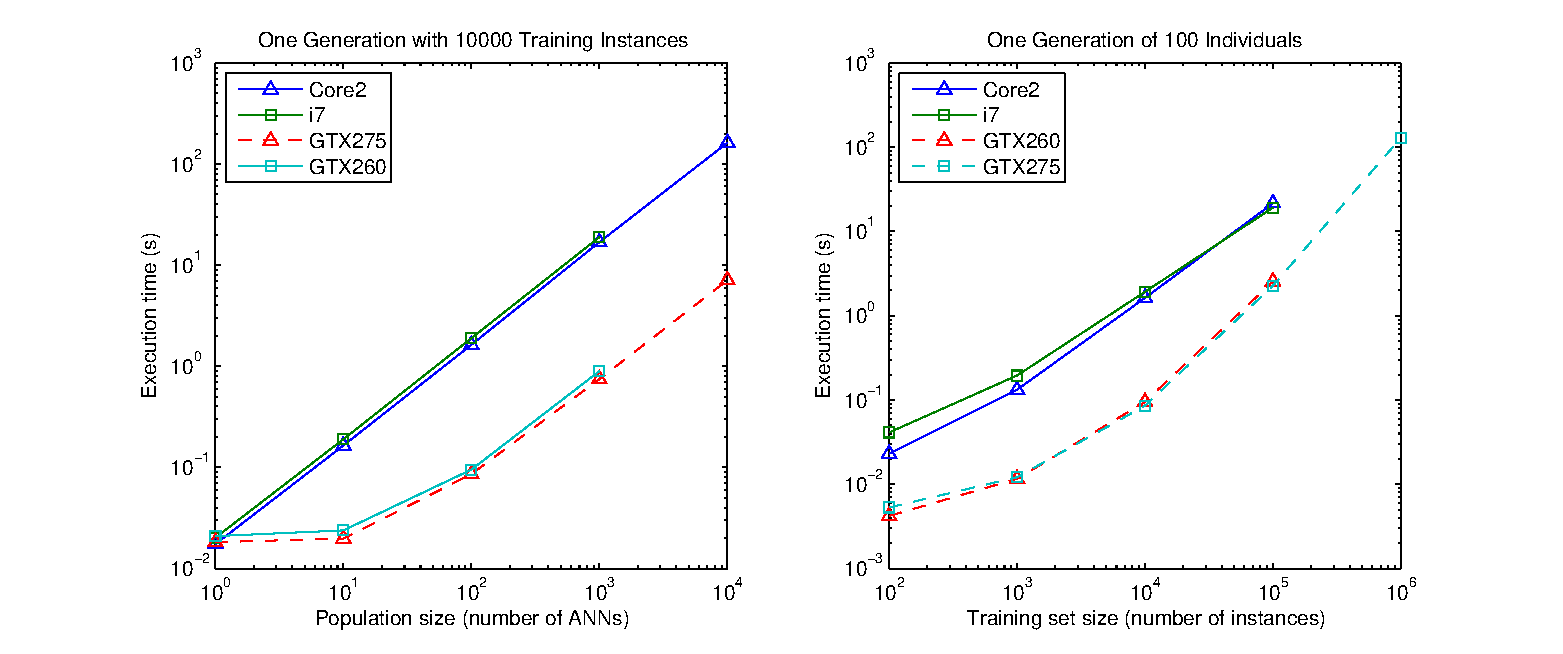
\includegraphics[width=\textwidth]{fig-performance}
	\caption{Training performance as a function of population size (left) and training set size (right). Note logarithmic axes.}
	\label{fig:training-performance}
\end{figure}

% ----------------------------------------------------------------------------
\subsection{Classifier Results} \label{results}
% ----------------------------------------------------------------------------
Filling this with text so that I can see what the document looks like when it is filled with text and to make sure that everything lines up nicely when it is full of text like this

% ############################################################################
\section{Conclusion} \label{concl}
% ############################################################################
Filling this with text so that I can see what the document looks like when it is filled with text and to make sure that everything lines up nicely when it is full of text like this

% ############################################################################
\section{Discussion} \label{disc}
% ############################################################################
Filling this with text so that I can see what the document looks like when it is filled with text and to make sure that everything lines up nicely when it is full of text like this

% ----------------------------------------------------------------------------
\subsection{Future Work} \label{future}
% ----------------------------------------------------------------------------
Filling this with text so that I can see what the document looks like when it is filled with text and to make sure that everything lines up nicely when it is full of text like this

% ############################################################################
% Bibliography
% ############################################################################
\bibliographystyle{plain}
\bibliography{bibliography}     %loads bibliography.bib

% ============================================================================
\end{document}
% ============================================================================
